\documentclass{article}

\usepackage{graphicx}
\usepackage{tikz}
\usepackage{tikzsymbols}
\usetikzlibrary{calc,patterns,shapes.geometric}
\pagestyle{empty}
\usepackage[margin=0pt]{geometry}
\geometry{papersize={14in,12in}}

\def\centerarc[#1](#2)(#3:#4:#5){\draw[#1] ($(#2)+({#5*cos(#3)},{#5*sin(#3)})$) arc (#3:#4:#5);}

\begin{document}
	\begin{figure}
		\centering
		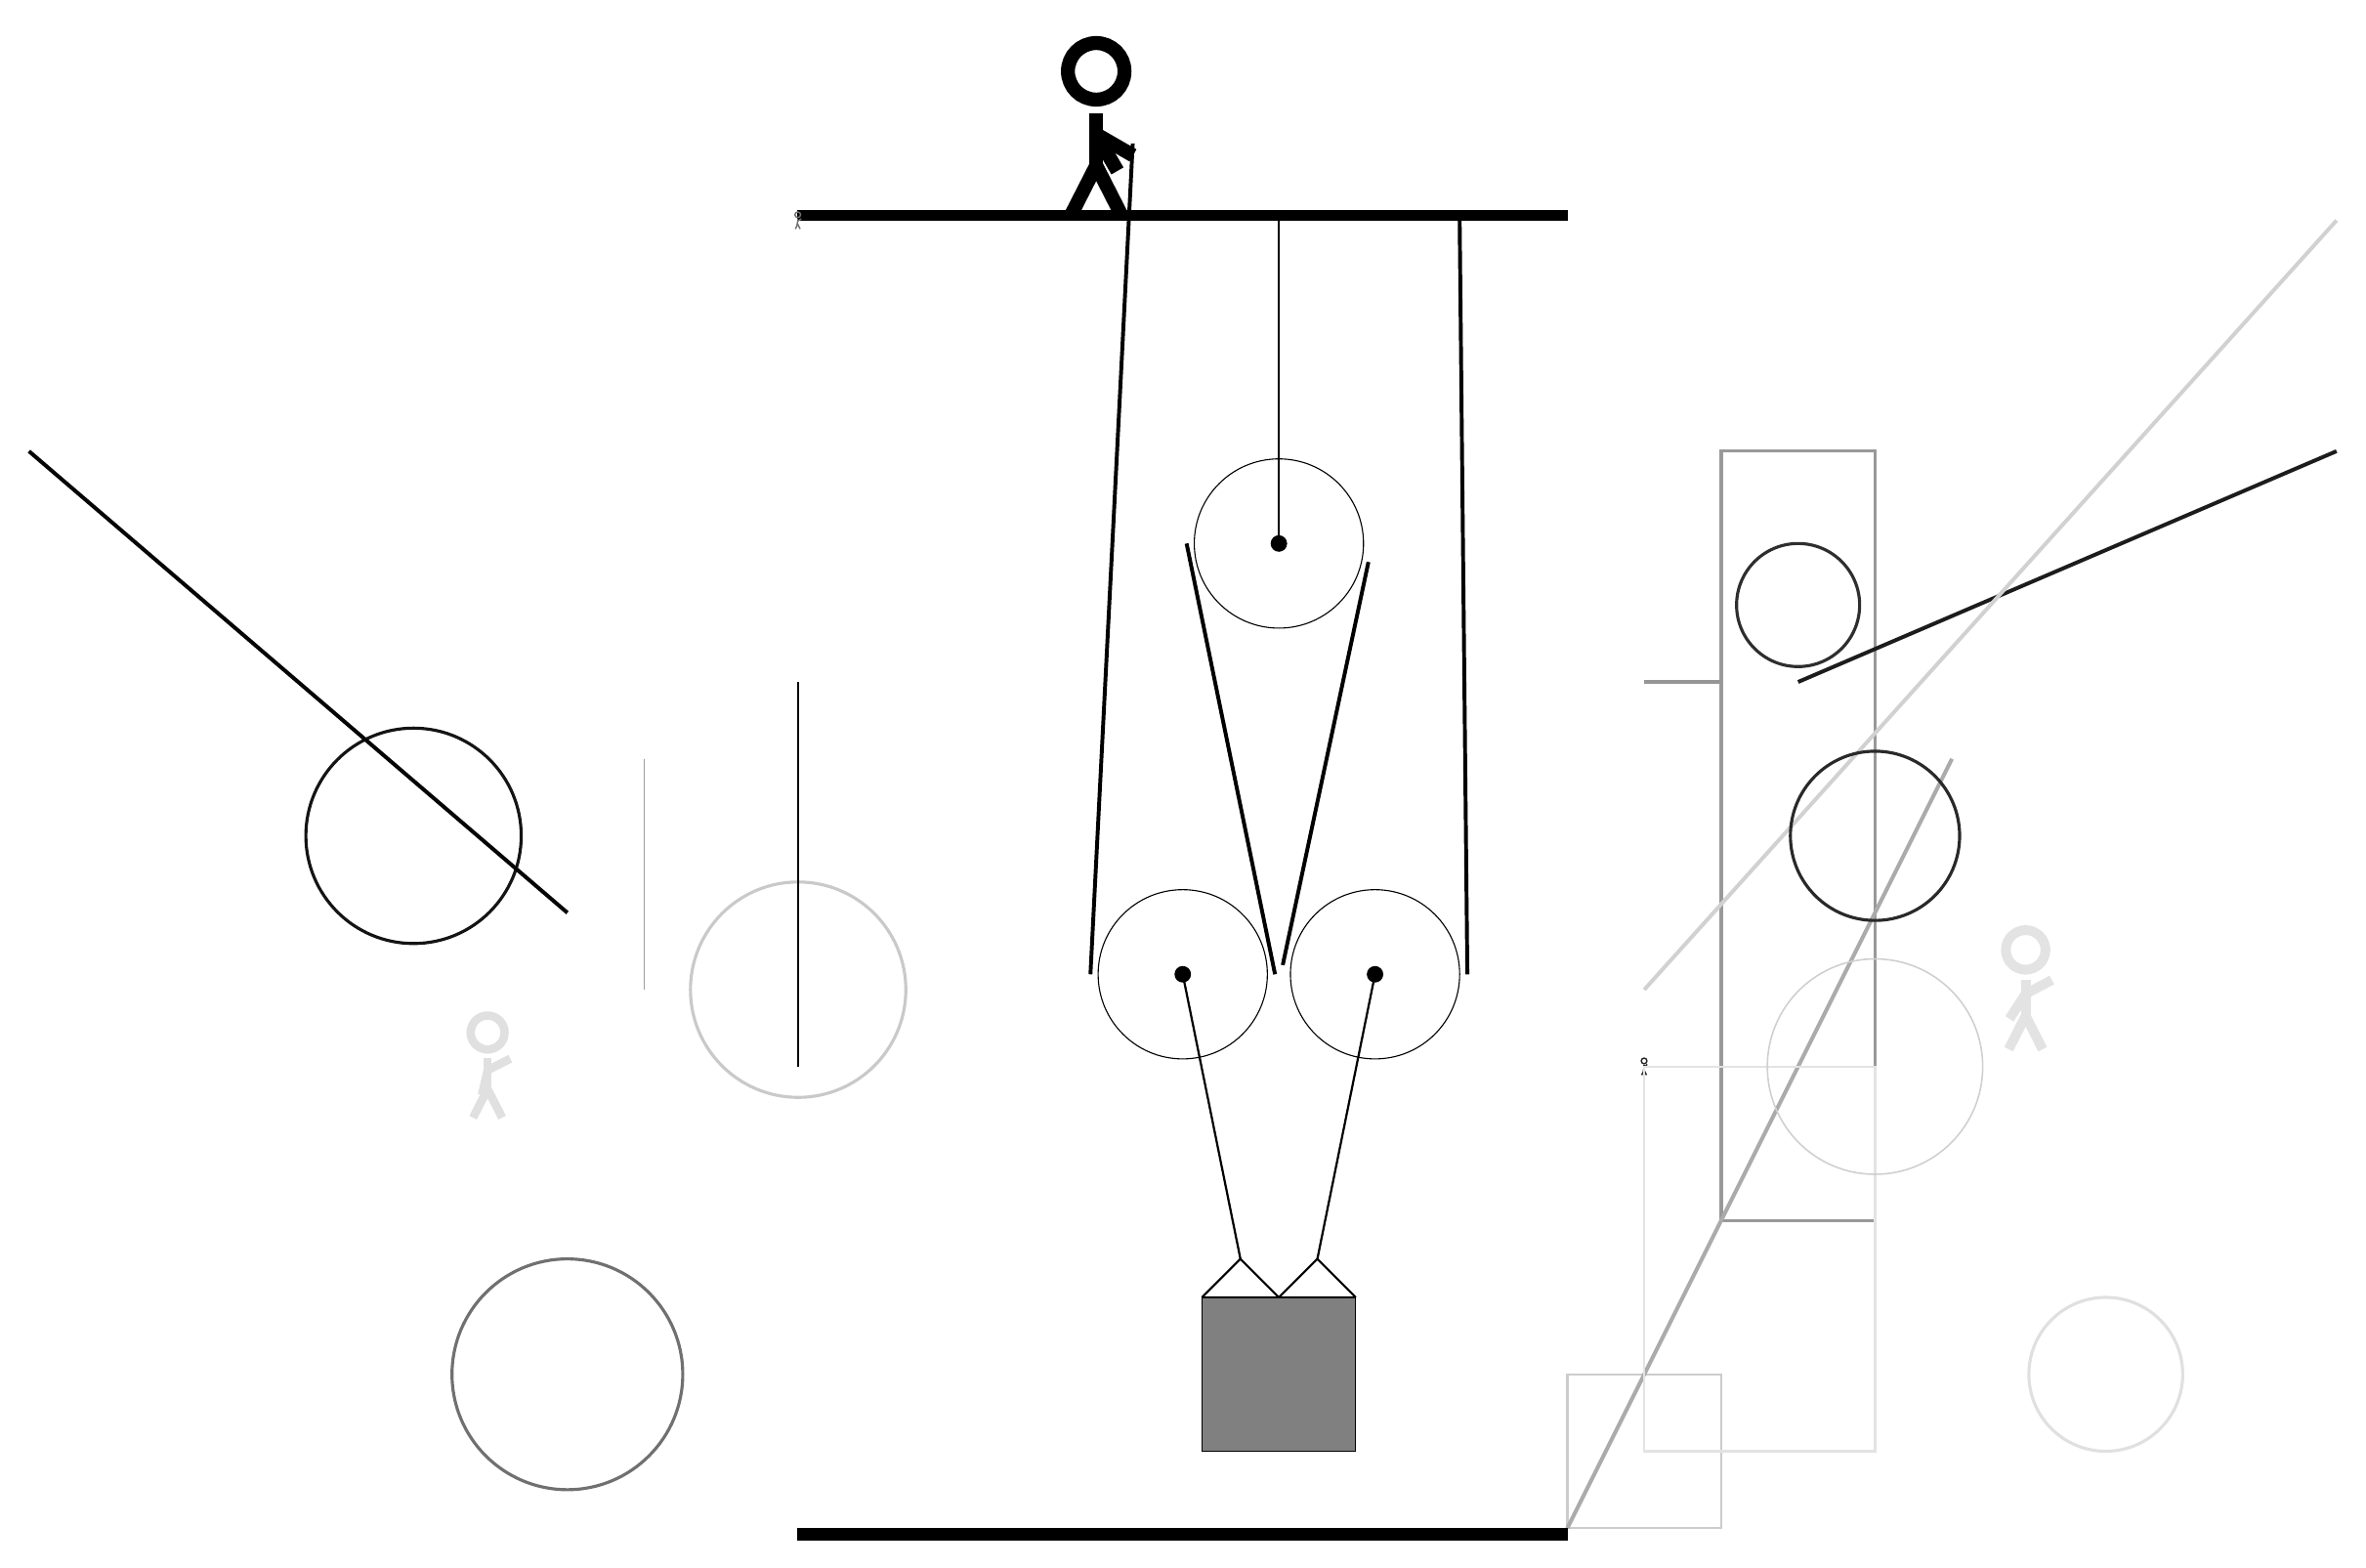
\begin{tikzpicture}
			%%%%% START %%%%%
			
			\draw[fill=black] (-4, 14) rectangle (6, 14.125);
			
			\draw (1, 4.2) circle (1.1);
			\draw[fill=black] (1, 4.2) circle (0.1);
			
			\draw (2.25, 9.8) circle (1.1);
			\draw[fill=black] (2.25, 9.8) circle (0.1);
			\draw[thick] (2.25, 9.8) -- (2.25, 14);
			
			\node[line width=0.5mm, color=black!11] at (12, 4) {\Strichmaxerl[7][57][28]};
			
			\draw [line width=0.4mm, color=black!82](9, 9) circle (0.8);
			\draw[line width=0.3mm, color=black!20] (6, -1) rectangle (8, -3);
			\draw[line width=0.4mm, color=black!40] (8, 11) rectangle (10, 1);
			
			\draw[line width=0.5mm, color=black!41](8, 8) -- (7, 8);
			
			\draw [line width=0.4mm, color=black!21](-4, 4) circle (1.4);
			\draw[line width=0.2mm, color=black!38] (-6, 4) rectangle (-6, 7);
			\draw [line width=0.4mm, color=black!56](-7, -1) circle (1.5);
			\draw[line width=0.5mm, color=black!89](9, 8) -- (16, 11);
			\node[line width=0.3mm, color=black!85] at (7, 3) {\Strichmaxerl[1][80][42]};
			
			\draw [line width=0.4mm, color=black!92](-9, 6) circle (1.4);
			\draw[line width=0.5mm, color=black!33](6, -3) -- (11, 7);
			\draw [line width=0.4mm, color=black!12](13, -1) circle (1.0);
			
			\draw[line width=0.3mm, color=black!11] (7, -2) rectangle (10, 3);
			\draw[line width=0.2mm, color=black!97] (-4, 3) rectangle (-4, 8);
			\node[line width=0.7mm, color=black!12] at (-8, 3) {\Strichmaxerl[6][77][27]};
			
			\node[line width=0.5mm, color=black!56] at (-4, 14) {\Strichmaxerl[1][80][31]};
			\draw[line width=0.5mm, color=black!18](7, 4) -- (16, 14);
			\draw [line width=0.4mm, color=black!84](10, 6) circle (1.1);
			\draw [line width=0.2mm, color=black!19](10, 3) circle (1.4);
			\draw[line width=0.5mm, color=black!98](-7, 5) -- (-14, 11);
			
			
			\draw (3.5, 4.2) circle (1.1);
			\draw[fill=black] (3.5, 4.2) circle (0.1);
			
			\draw[thick] (3.5, 4.2) -- (2.75, 0.5);
			\draw[thick] (1, 4.2) -- (1.75, 0.5);
			\draw[thick]  (1.25, 0) -- (1.75, 0.5) -- (2.25, 0);
			\draw[thick]  (2.25, 0) -- (2.75, 0.5) -- (3.25, 0);
			\draw[fill=black!50] (1.25, 0) rectangle (3.25, -2);
			
			\draw[line width=0.5mm] (0.35, 15) --  (-0.2, 4.2);
			\centerarc[line width=0.5mm](1, 4.2)(180:360:1.2000000000000002);
			\draw[line width=0.5mm] (2.2, 4.2) -- (1.05, 9.8);
			\centerarc[line width=0.5mm](2.25, 9.8)(-20:180:1.2000000000000002);
			\draw[line width=0.5mm](3.414, 9.56) -- (2.3, 4.32);
			\centerarc[line width=0.5mm](3.5, 4.2)(160:360:1.2000000000000002);
			\draw[line width=0.5mm](4.7, 4.2) -- (4.6, 14);
			
			\node at (-0.07, 15.2) {\Strichmaxerl[10][120][-30]};
			
			\draw[fill=black] (-4, -3) rectangle (6, -3.15);
			
			%%%%% END %%%%%
		\end{tikzpicture}
	\end{figure}	
\end{document}